% comment
\documentclass[18pt,a4paper]{article}


\usepackage{biblatex}
\usepackage{graphics}
\usepackage{color}
\usepackage{multicol}
\usepackage{multirow}
\usepackage[utf8]{inputenc}
\usepackage{amsmath}

\addbibresource{references.bib}

\author{Mahdi Hasnat Siyam}
\title{Intro to {\LaTeX}}
\date{\today}

\begin{document}
\maketitle   
\tableofcontents
\pagebreak

\section{Introduction}
This is the introduction section.Citing \cite{adams1995hitchhiker} \\
Lists can be three types
This is a itemize list
\begin{itemize}
    \item Itemize
    \begin{itemize}
        \item nestet item 1
        \item nestet item 2
    \end{itemize}
    \item Enumerate
    \item Description
\end{itemize}
This is a enumerate list
\begin{enumerate}
    \item enum 1
    \begin{enumerate}
        \item nested enum 1
        \item nested enum 2
    \end{enumerate}
    \item enum 2
    \item enum 3
\end{enumerate}
This is a description list
\begin{description}
    \item[Number 1] desc 1
    \item[Number 2] desc 2
\end{description}

\subsection{Subsection x.y}
This is a subsection.
\par
This is a demo line for new line demonstration
\subsubsection{Subsubsection x.y.z}
This is a subsubsection
\subsection{Another subsection x.y}
This is another subsection
\newline
\textbf{This is bold \emph{statement}.}
\newline
\textit{This is italic \emph{statement}.}
\newline
{\color{red} This is colored \emph{text}.}
\newline
\large{This sentence is large}
\newline
\huge{This sentence is huge.}
\newline
\small{This sentence is small.}
\section*{Body Paragraph}
This is body paragraph
\section{Figure example}
\begin{figure}[h]
    \centering
    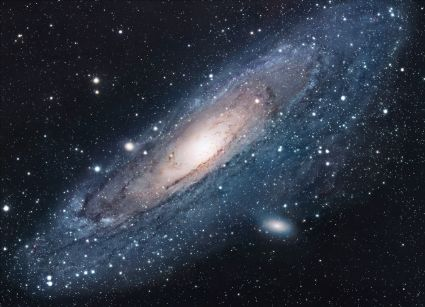
\includegraphics{universe.jpg}
    \caption{Caption}
    \label{fig:fig_1}
\end{figure}

\ref{fig:fig_1} is a figure
\section{Table}
\begin{tabular}{|c|c|c|}
    \hline
    
    \multicolumn{3}{|c|}{Number}  \\
    \cline{2-2}
    \multirow{2}{*}{text} &5 & 6\\
    \cline{2-3}
     & 5 & 6\\
    \hline
    \multicolumn{2}{|c|}{ \multirow{2}{*}{2x2} }& 3 \\
    \cline{3-3}
    \multicolumn{2}{|c|}{ }& 6 \\
    \hline
    
\end{tabular}

\section{Equation and Math Mode}
Equations goes here
\newline
This ``\%equation" will not start in new block $a+a = 2a$\\
new block eqn $$ a+a = 2a $$
eqn with number
\begin{equation}
    a+a = 2a^b
\end{equation}

\subsection{sub script and super script}
Superscript: $a^b$ ,$a^{in}$ , $a^{i^n}$ \\
Subscript: $a_b$,$a_{in}$ ,$a_{i_n}$
\subsection{Example}
Comparison : $<$ , $>$ , $\leq$ , $\geq$ \\ 
Set Operation : $A \cap B$ , $A \cup B $ \\
Fraction : $\frac{a}{b}$ , ($\frac{a}{b}$) , $(\frac{a}{b})$ , $\left(\frac{a}{b}\right)$\\
Equation : $P(A) = \sum P\left( \{e_1,...,e_N \} \right) =  \binom{N}{k} p^k p^{N-k} $
\printbibliography

\section{Conclusion}
This is the concluding section.
\end{document}